\chapter{Introduction}
\section{Topic}
IoT devices are on the rise and it is hard to imagine our everyday life without them. They make many everyday tasks easier, collect information or connect us with other people. New applications for these small and often practical devices are being added every day.
\newline
However, the majority of these IoT devices have a very large weak point. The data exchange of the IoT devices is often handled by the manufacturer of the devices. This means that if a manufacturer goes bankrupt, the IoT devices from this manufacturer often become useless, as the data exchange between the devices can no longer take place.
\newline
My goal is to start with exactly this rough problem. 
In this work we want to work out a way to break the dependency of the IoT devices to the manufacturers. It should be possible for us to operate our IoT devices without the communication via the manufacturer, and thus free us from the risk of a complete failure of our IoT infrastructure in the event of bankruptcy of the manufacturer. We will thus outsource the communication of the IoT devices to a broker. This broker will replace the manufacturer as a communication node and it should be possible for us to operate this broker locally (in the same network).
\newline
In this paper I will show you a more detailed insight into our new communication line, and I will also provide you with the most important information about the selected broker. 
\newpage
\section{What is a Broker}
A broker is a server or service that caches data from clients and makes it available for retrieval. It therefore represents the communication interface between two end devices. In our case, the broker is the data node between the IoT device that measures the patient's vital signs and the end device that makes the measured data available to the medical staff for viewing.
Data exchanged through a broker is often public and available for all to see. The challenge of storing data anonymously and making it unrecognizable so that it cannot be read by third parties is mandatory for the use of a broker when sensitive data is involved.

\section{Freenet}
Freenet is free software which lets you anonymously share files, browse and publish "freesites" (web sites accessible only through Freenet) and chat on forums, without fear of censorship. Freenet is decentralised to make it less vulnerable to attack, and if used in "darknet" mode, where users only connect to their freinds, is very difficult to detect.
\newline
Communications by Freenet nodes are encrypted and are routed through other nodes to make it extremely difficult to determine who is requested the information and what its content is.
\newline
Users contribute to the network by giving bandwidth and a portion of their hard drive (called the "data store") for storing files. Files are automatically kept or deleted depending on how popular they are, with the least popular being discared to make way for newer or more popular content. Files are encrypted, so generally the user cannot easily discover what is in his datastore, and hopefully can't be held accountable for it. Chat forums, websites, and search functionality, are all built on top of this distributed data store.\cite{freenet}
\newpage
\section{Hardware}
For the implementation of this work, different hardware is used. The following hardware is used:
\newline
\renewcommand\tabularxcolumn[1]{>{\centering\arraybackslash}m{#1}}
\newcommand*\tablehead[1]{\multicolumn{1}{c}{\textbf{#1}}}
\begin{tabularx}{\textwidth}{p{4cm}|p{10cm}}
\toprule
Hardware  & Overview\\ 
\midrule 
\raisebox{\ht\strutbox-\height}{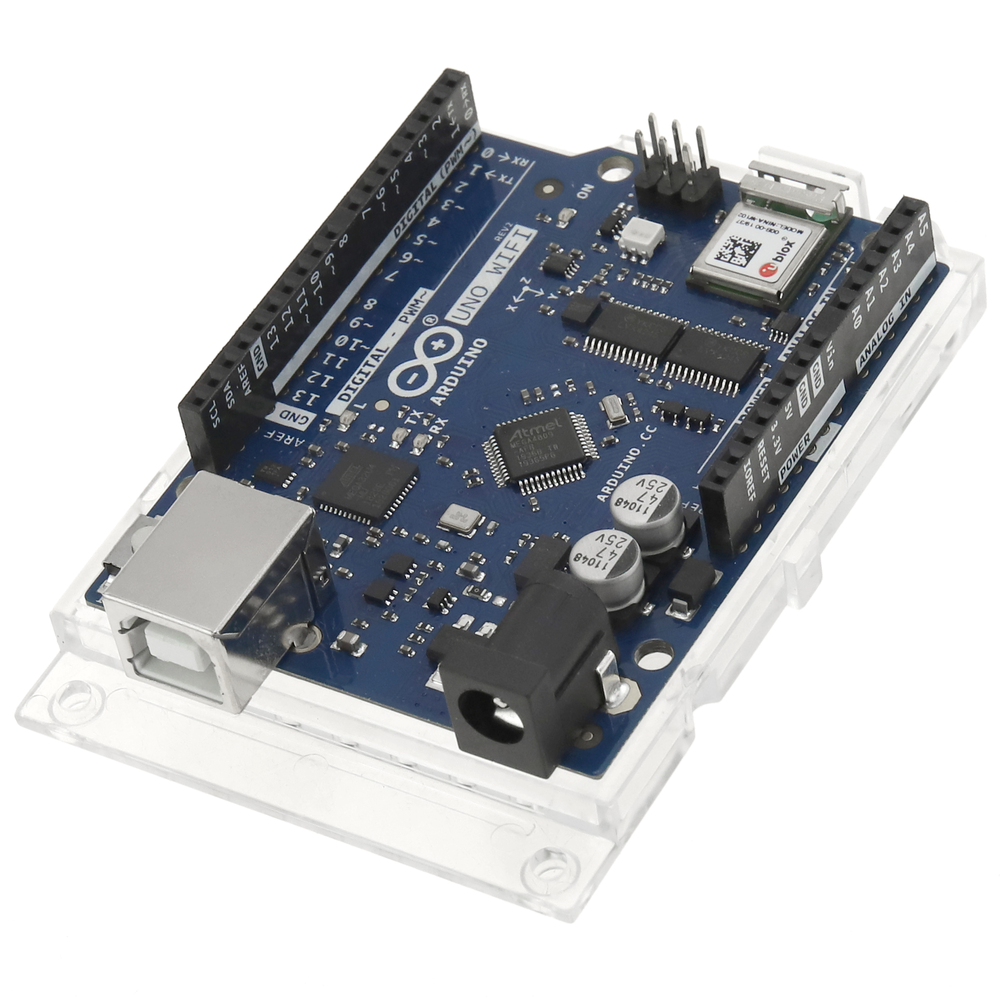
\includegraphics[width=0.25\textwidth]{resources/images/arduino.jpg}} & The arduino UNO Wifi Rev.2 is a very basic entry to IoT. It offers many different possibilities to build and expand it's functions. 
     \newline
     The Ardunino UNO Wifi Rev.2 has 14 digital input/output pins and 6 analog inputs. With its secure ECC608 crypto chip accelerator it is possible to directly connect the Arduino UNO Wifi Rev.2 to a Wifi network of your choice. \\
\addlinespace
\hline
\addlinespace
\raisebox{\ht\strutbox-\height}{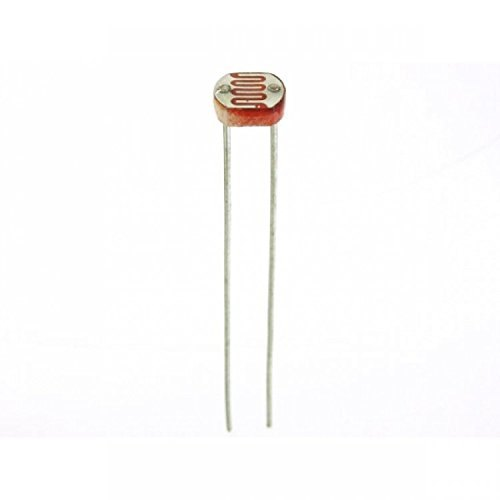
\includegraphics[width=0.25\textwidth]{resources/images/ldr.jpg}} & LDR's or Light Dependent Resistors are used in light/dark sensor circuits. The resistance of LDR normally is very high, sometimes as high as 1 Mega ohms, if they then get illuminated the resistance drops dramatically. \\
\addlinespace
\hline
\addlinespace
\raisebox{\ht\strutbox-\height}{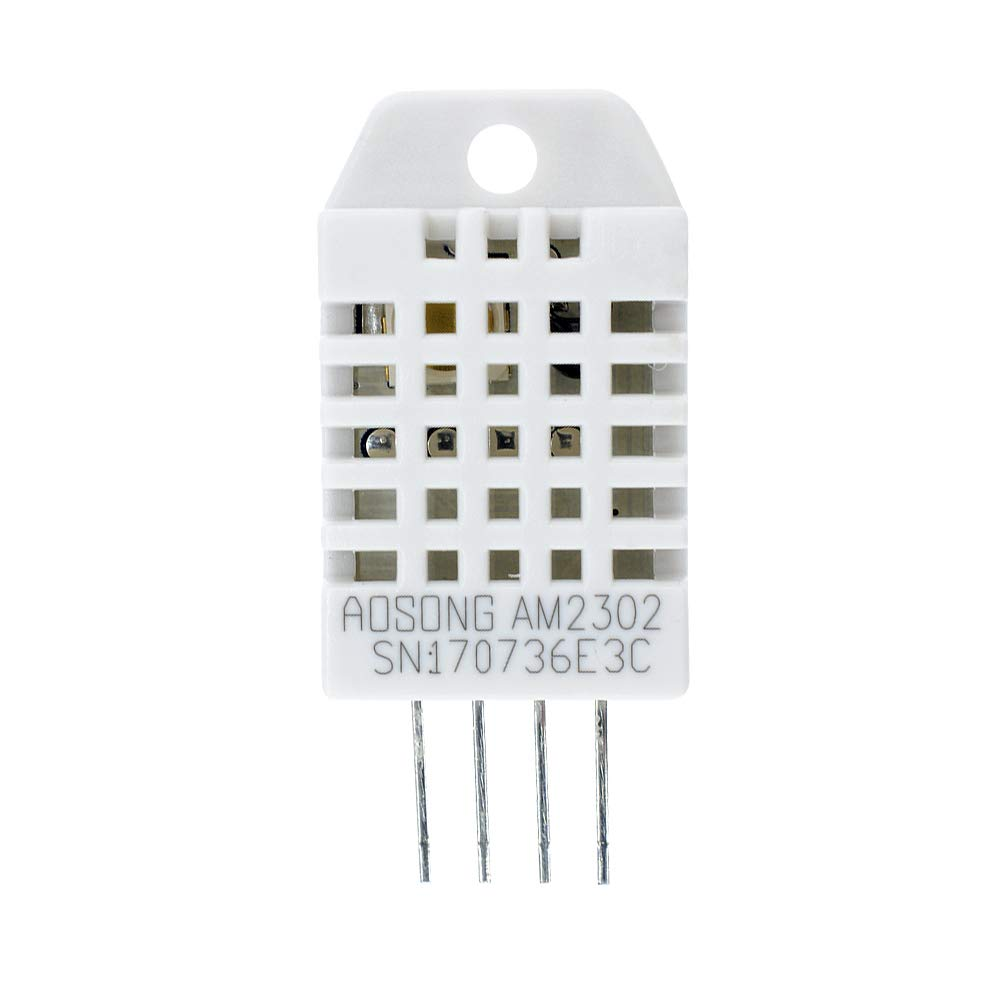
\includegraphics[width=0.25\textwidth]{resources/images/dt22.jpg}} & The DHT22 is low cost easy to use humidity and temperature sensor. It can measures humidity from 0-100\% with and accuracy of 2-5\% and the temperature from -40 to 80°C with accuracy +-0.5°C\\
\addlinespace
\hline
\addlinespace
\raisebox{\ht\strutbox-\height}{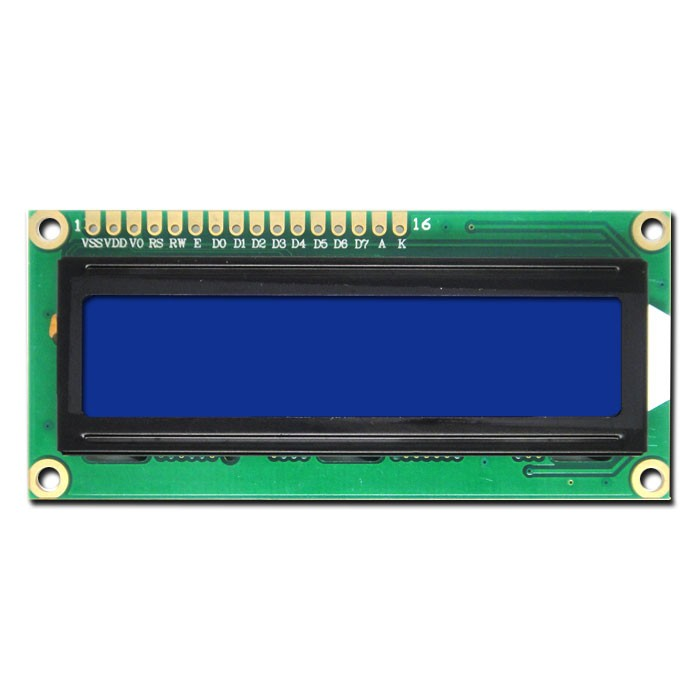
\includegraphics[width=0.25\textwidth]{resources/images/lcdDisplay.jpg}} &  The LCM1602C is a 2x16 LCD display which can be used to display information up to 32 characters over 2 lines.\\
\bottomrule
\end{tabularx}